\let\lesson\undefined
\newcommand{\lesson}{\phantomlesson{Bài 10.}}
\setcounter{section}{2}
\section{Bài tập trắc nghiệm}
\begin{enumerate}[label=\bfseries Câu \arabic*:,leftmargin=1.5cm]
	\item \mkstar{2}\\
	{Một chiếc xe đang chuyển động với tốc độ không đổi, trên mui xe có đặt một thùng hàng. Khi xe va vào vật cản thì thùng hàng bị hất văng về trước. Điều lý giải nào sau đây là phù hợp?
		\begin{center}
			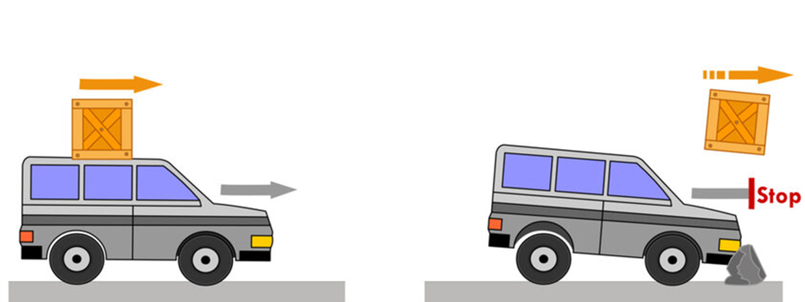
\includegraphics[width=0.4\linewidth]{../figs/VN10-2023-PH-TP015-P-1}
		\end{center}
		\begin{mcq}
			\item Khi xe va vào đá, xe tác dụng một lực $\overrightarrow{F}$ hướng về phía trước lên thùng hàng làm cho thùng hàng chuyển động về trước.
			\item Phản lực do mui xe tác dụng lên thùng hàng làm thùng hàng chuyển động về trước.
			\item Thùng hàng chuyển động cùng vận tốc với xe, khi xe va chạm và dừng lại thì thùng hàng vẫn tiếp tục chuyển động theo quán tính.
			\item Phản lực do hòn đá tác dụng lên xe trong quá trình và chạm làm cho thùng hàng chuyển động về trước.
		\end{mcq}
	
}
\hideall{
\textbf{Đáp án: C.}
}

\item \mkstar{2}\\
{Một xe ô tô đang chuyển động thẳng với vận tốc không đổi $\SI{20}{\meter/\second}$. Hợp lực tác dụng lên xe ô tô có độ lớn bằng
	\begin{mcq}(4)
		\item $\SI{20}{\newton}$.
		\item $\SI{0}{\newton}$.
		\item $\SI{10}{\newton}$.
		\item $\SI{-20}{\newton}$.
	\end{mcq}

}
\hideall{
\textbf{Đáp án: B.}
}


\item \mkstar{2}\\
{Chọn phát biểu đúng.   
	\begin{mcq}
		\item Khi vật bị biến dạng hoặc vận tốc của vật thay đổi thì chắc chắn đã có lực tác dụng lên vật. 
		\item Vật luôn chuyển động cùng hướng với hướng của ngoại lực tác dụng. 
		\item Khi một vật đang đứng yên chịu tác dụng của lực thì vật bắt đầu chuyển động, do đó lực là nguyên nhân gây ra chuyển động.
		\item Nếu tổng hợp lực tác dụng lên vật bằng không thì vật phải đứng yên. 
	\end{mcq}

}
\hideall{
\textbf{Đáp án: A.}
}

\item \mkstar{2}\\
{Một chiếc xe đang chạy với tốc độ $\SI{50}{\kilo\meter/\hour}$. Nếu bỗng nhiên các lực tác dụng lên nó mất đi thì   
\begin{mcq}
	\item xe dừng lại ngay.   
	\item xe tiếp tục chuyển động theo hướng cũ với vận tốc $\SI{50}{\kilo\meter/\hour}$.
	\item xe đổi hướng chuyển động.  
	\item xe chuyển động chậm dần rồi dừng lại.   
\end{mcq}
}
\hideall{
\textbf{Đáp án: B.}
}

\item \mkstar{2}\\
{Trên một chiếc xe buýt đang chuyển động thẳng đều, bạn Sang ném quả táo theo phương thẳng đứng, khi quả táo rơi xuống thì
	\begin{mcq}
		\item quả táo rơi về phía trước bạn Sang do quán tính.
		\item quả táo rơi về phía sau bạn Sang do quán tính.
		\item quả táo rơi trở lại tay bạn Sang vì trong hệ quy chiếu gắn với xe đang chạy thẳng đều quả táo chỉ chịu tác dụng của trọng lực theo phương thẳng đứng.
		\item chưa thể xác định được vì phương chuyển động của quả táo còn phụ thuộc vào hướng chuyển động của xe.
	\end{mcq}

}
\hideall{
\textbf{Đáp án: C.}
}

\item \mkstar{2}\\
{Hiện tượng nào sau đây không thể hiện tính quán tính?
	\begin{mcq}
		\item Quả bóng bị nảy lên sau khi đập vào sàn nhà.
		\item Người ngồi trên xe bị ngã về sau khi xe đột ngột tăng tốc.
		\item Các giọt nước bị văng ra khi ta vẫy mạnh một chiếc khăn ướt.
		\item Khi phanh gấp, xe vẫn chạy thêm một đoạn nữa trước khi dừng lại.
	\end{mcq}

}
\hideall{
\textbf{Đáp án: A.}
}

\item \mkstar{3}\\
{Hành khách ngồi trên xe ôtô đang chuyển động, xe bất ngờ rẽ sang phải. Theo quán tính hành khách sẽ
	\begin{mcq}(2)
		\item nghiêng sang phải.  
		\item nghiêng sang trái
		\item ngã người về phía sau.        
		\item chúi người về phía trước.
	\end{mcq}

}
\hideall{
\textbf{Đáp án: B.}
}

\item \mkstar{3}\\
{Trong các ví dụ sau đây, ví dụ nào không liên quan đến quán tính?
	\begin{mcq}
		\item Khi đi trên đường trơn trượt, người ta có xu hướng bị ngã về phía trước.
		\item Lưỡi búa được tra vào cán khi gõ cán búa xuống nền.
		\item Chiếc xe tải chở đầy hàng hoá khó dừng lại khi phanh hơn so với chiếc xe tải không chở hàng.
		\item Khi chúng ta bước từ thuyền lên bờ, thuyền bị lùi về phía sau.
	\end{mcq}

}
\hideall{
\textbf{Đáp án: D.}
}
\end{enumerate}
\section{Bài tập tự luận}

\begin{enumerate}[label=\bfseries Bài \arabic*:,leftmargin=1.5cm]
	\item \mkstar{1}\\
	{Khi một quyển sách nằm yên trên mặt bàn, ta có thể kết luận rằng quyển sách không chịu tác dụng của lực nào được không? Giải thích.
	
}
\hideall{
Không. Vật có thể chịu tác dụng của nhiều lực tác dụng, nhưng các lực này là cân bằng nhau.
}

\item \mkstar{1}

{
	Để tra đầu búa vào cán, nên chọn cách nào dưới đây? Giải tính tại sao?
	\begin{center}
		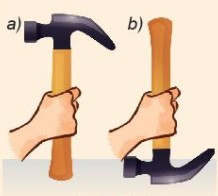
\includegraphics[scale=1]{../figs/VN10-2022-PH-TP017-1.jpg}
	\end{center}
	\begin{enumerate}[label=\alph*)]
		\item Đập mạnh cán búa xuống đất như hình a.
		\item Đập mạnh đầu búa xuống đất như hình b.
	\end{enumerate}
}

\hideall{
	
	Ta nên chọn cách đập mạnh cán búa xuống đất như Hình a. Vì khi đập cán búa xuống đất, khi chạm đất thì cán búa dừng lại đột ngột, theo quán tính đầu búa vẫn có xu hướng bảo toàn vận tốc cả về hướng và độ lớn nên vẫn tiếp tục đi xuống. Do vậy, đầu búa sẽ dễ tra vào cán hơn và chắc chắn hơn.
}

\item \mkstar{2}\\
{Khi một vật được thả từ đỉnh một máng nghiêng tới chân máng thì vật chỉ chuyển động trên máng ngang một đoạn rồi dừng lại. Trong trường hợp này có phải định luật I Newton không đúng hay không? Giải thích.

}
\hideall{
Không phải định luật I Newton không đúng mà do có ma sát.
}

\item \mkstar{3}\\
{Một em bé ngồi trên xe đẩy nói rằng, mẹ dừng xe đột ngột làm đồ chơi treo ở đầu xe bay vào em. Em bé nói đúng hay sai?

}
\hideall{
Em bé nói sai. Vì khi mẹ dừng xe đột ngột thì đồ chơi treo ở đầu xe sẽ bay về phía trước.
}

\item \mkstar{3}\\
{Hãy giải thích sự cần thiết và lợi ích của túi khí được trang bị trong ô tô.

}
\hideall{
Trong tình huống xảy ra va chạm giao thông, do xe đột ngột giảm tốc nên người ngồi trong xe có xu hướng bị chúi về trước. Túi khí được bơm phồng gần như ngay lập tức với thời gian tính bằng mili giây, các bộ phận quan trọng trên cơ thể người ngồi trên xe như đầu, lồng ngực, tay, \dots sẽ được túi khí bảo vệ do chỉ va chạm với túi khí mà không va chạm với thành xe.
}
\end{enumerate}


